\documentclass{standalone}
% Option-clash probe: circuitikz is option-sensitive and deliberately
% excluded from the fmt preload set (the preload convention loads
% packages classless with no options), so this \usepackage[european]{...}
% must load at RUNTIME with the option effective — the resistor below
% takes the European rectangle shape only because the option was
% processed at runtime. If a future preload set wrongly included
% circuitikz, the same line becomes a hard "Option clash" error and the
% gate catches it. tikz-cd likewise loads at runtime (excluded from the
% preload set on purpose); the cascaded superscript sweeps cmsy script
% sizes.
\usepackage[european]{circuitikz}
\usepackage{tikz-cd}
\begin{document}
\begin{tikzcd} A \arrow[r, "\times"] & B^{C^{A \times B}} \end{tikzcd}
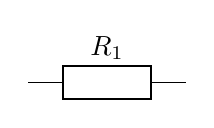
\begin{tikzpicture}
\draw (0,0) to[R=$R_1$] (2,0);
\end{tikzpicture}
\end{document}
